\documentclass{scrartcl}
\usepackage[a4paper, total={7in, 9.5in}]{geometry}
\usepackage{amsmath,amsthm,amssymb}
\usepackage{fontspec}
\usepackage{graphicx}
\usepackage{xcolor}
\usepackage{enumitem}
\usepackage{placeins}
\usepackage[most]{tcolorbox}
\usepackage{tikz}
\usepackage[font=small, justification=centering, format=plain, indention=0pt]{caption}
\usepackage[indent]{parskip}
\usepackage{unicode-math}
\usepackage{array}
\usepackage{multirow}
\usepackage{booktabs}



\setmainfont{tex-gyre-pagella.regular}[
    Path=../fonts/,
    Extension=.otf,
    BoldFont=tex-gyre-pagella.bold,
    ItalicFont=tex-gyre-pagella.italic,
    BoldItalicFont=tex-gyre-pagella.bold-italic,
]
\setmathfont{texgyrepagella-math}[
    Path=../fonts/,
    Extension=.otf,
]

\KOMAoptions{DIV=14}
\KOMAoptions{fontsize=12pt}
\KOMAoptions{BCOR=0mm}

\def\eps{\varepsilon}
\def\vphi{\varphi}
\def\bR{\mathbb R}
\def\bC{\mathbb C}
\def\bE{\mathbb E}
\def\bP{\mathbb P}

\DeclareMathOperator*{\argmax}{arg\,max}
\DeclareMathOperator*{\argmin}{arg\,min}

\newtheorem{Theorem}{Theorem}
\newtheorem{Proposition}{Theorem}
\newtheorem{Lemma}[Theorem]{Lemma}
\newtheorem{Corollary}[Theorem]{Corollary}

\theoremstyle{definition}
\newtheorem{Definition}[Theorem]{Definition}

\setlength\parskip{4pt}

\renewcommand*{\thefootnote}{[\arabic{footnote}]}


\begin{document}
\begin{titlepage}
    \noindent
    \begin{tabular}{@{}m{0.3\textwidth}@{} m{0.4\textwidth}@{} m{0.3\textwidth}@{}}
        \includegraphics[width=3cm]{imgs/insat} &
        \centering
            \textsc{Carthage University}\\[.2cm]
            \textsc{National Institute of Applied}\\
            \textsc{Sciences and Technology} &
        \raggedleft
        \includegraphics[width=3cm]{imgs/ucar}
    \end{tabular}
    \vfill
    
    \centering
        \textsc{\LARGE Professional Personal Project}\\[.7cm]
        \textsc{\large as part of the}\\[.7cm]
        \textsc{\Large National Engineering Diploma}\\[.3cm]
        \textsc{\large in Networks and Telecommunications}
    \vfill
    
    \rule{\linewidth}{0.2 mm}\\[1 cm]
    {\huge \bfseries Ultrasound-Based Indoors Real-Time Location System}\\[.7 cm]
    \rule{\linewidth}{0.2 mm}
    \vfill
    
        {\large\bfseries Authors:}\\[.2cm]
        {\large \textsc{Ben Fraj} Mohamed Amine, \hspace{1.5em} \textsc{Brahim} Amine,}\\[.2cm]
        {\large \textsc{Eladab} Youssef, \hspace{1.5em} \textsc{Ilehi} Alaa}
        \\[1cm]
    {\large\bfseries Supervisor:}\\[.2cm]
    {\large \textsc{Miled Souid} Wided}\\[.2cm]
    \vfill
    {\large June 2026}
\end{titlepage}

\large

% Acknowledgements Page
\clearpage
\thispagestyle{empty}

\begin{center}
  {\Large\rmfamily\bfseries Acknowledgments}
\end{center}

We would like to extend our thanks towards...

% Abstract Page
\clearpage

\begin{center}
  {\Large\bfseries Abstract}
\end{center}

\vspace{1em}

\noindent
Your abstract text...

\pagebreak
\tableofcontents

\pagebreak
\section{Introduction}
Intro text...

% Background section goes in background.tex 
\section{Background}
Talk about different kinds of RTLSs and SLAM here...


% Math section goes in math.tex
\section{Mathematical Foundations}
Throughout this paper, we exclusively work with ToF-based methods. As ToF information can be trivially equated to travel distance information, we use the latter as the building block for our mathematical modeling.

In order to build up a solid mathematical model for our positioning problem, we work as all applied mathematicians do: build a simple toy model, and slowly expand upon it until we obtain a ``reasonable'' approximation of reality.
For this purpose, we build our base toy model on two assumptions: the target to track is a single point in space, and the distance measurements exactly equal to the true distances.


Once we have mastered this toy model, we relax the second hypothesis into one that better approximates reality: that of additive gaussian noise. The first assumption, however, is difficult to relax, hence our treatment will be limited to situations where ``the target is a point'' is a reasonable approximation of reality; that is, when the target is judged relatively small in dimensions.

\subsection{Working with Infallible Measurements}
We are interested in the problem of recovering the coordinates of a target point $t$ in $m$-dimensional Euclidian space, given its respective distances $d_1, \dots, d_n$ to a set of anchor points $a_1, \dots, a_n$. In RTLS applications, $m$ is taken to be either 2 or 3.

Our initial goal is to identify sufficient conditions on the number and geometry of the anchors that guarantee the solvability of this problem. Where necessary, we will treat the problems of positioning a target within a confined region (as is the case in indoor RTLSs, as well as some outdoor ones), and an unconfined target separately.

Given our assumption of measurement infallibility, the problem can be formulated purely in terms of vectors and scalars, and we will show that the solvability question can be explored with the tools of linear algebra, calculus and topology alone. Moreover, we will present some of the possible solution strategies.

We choose to do our investigation by exploring the different possibile values $n$ can take on: $n<m$, $n=m$, and $n>m$.

\subsubsection{The case of $n<m$}
Be it in the confined formulation of the positioning problem or the unconfined one, we generally assume the region wherein the target lies --- which we dub ``positioning region" --- to be open.

In the latter case, this is because it's exactly the whole of $\bR^m$. And in the former case, this is because the boundary of said region is considered to be impenetrable to the target (i.e. the target can never truly lie on the boundary).

Leveraging this fact, we invoke a result from topology: the invariance of domain theorem.

\begin{Theorem}[Invariance of Domain]
Let $U\in\bR^p$ be open and non-empty, $f:U\to\bR^p$. If $f$ is injective and continuous, then $V:=f(U)$ is open and $f:U\to V$ is a homeomorphism.
\end{Theorem}

The proof of the above theorem is too involved for our purposes, and hence we forego it. What truly interests us is the following corollary of the theorem.

\begin{Corollary}
    Let $p>q$, and let $U\subset\bR^p$ be open and non-empty. Then there exists no function $f:U\to\bR^q$ that is injective and continuous.
\end{Corollary}

\begin{proof}
We reason by contradiction. Let $U$ be a non-empty open in $\bR^p$, and suppose there exists a function $f:U\to\bR^q$ injective and continuous.

Since $p>q$, we consider the standard embedding $\vphi$ of $\bR^q$ into $\bR^p$:
\begin{align*}
    \vphi: \bR^q &\longrightarrow \bR^p \\
    (x_1, \dots, x_q) &\longmapsto (x_1, \dots, x_q, 0, \dots, 0)
\end{align*}
As $\vphi$ is injective and continuous, the same is the case for $\vphi\circ f: U\to\bR^p$. Then $\vphi\circ f(U)$ is open by Invariance of Domain.

Yet, picking an arbitrary $v\in\vphi\circ f(U)$, any open $p$-ball about $v$ must include, in particular, a point of non-zero $p$-th coordinate. However, such a point cannot be in the image of $\vphi$, and hence $\vphi\circ f(U)$ is not open; reaching a contradiction.

Thus such an $f$ cannot exist.
\end{proof}

To apply this corollary to our use case, we denote by $U$ the open region in $\bR^m$ wherein lies our target $t$.

If we wish for the coordinates of $t$ to be uniquely recoverable from its distances, we naturally require that
\begin{align*}
    f: U &\longrightarrow\bR^n \\
    x &\longmapsto (\Vert x-a_1\Vert,\dots,\Vert x-a_n\Vert)
\end{align*}
be injective. Further, by continuity of the Euclidian norm $\Vert \cdot\Vert$, $f$ is continuous. Since $m>n$, $f$ cannot exist with those conditions by our corollary.

To see why this makes sense, let's consider the case of a 2D RTLS, where $m=2$ and $n=1$. The information $\Vert t-a_1\Vert=d_1$ is equivalent to $t\in S^1(a_1, d_1)$\footnote{$S^d$ denotes the topolgist's $d$-sphere, or equivalently the analyst's $(d+1)$-sphere: $$S^d(p,q) = \{ x\in\bR^{d+1}\mid \Vert x-p\Vert=q \}$$}
the circle of radius $d_1$ and of center $a_1$.

By openness of $U$, the positioning region, there exists an open ball about $t$ contained in $U$, and hence, in particular, an open arc of the circle. As a result, all points on the open arc are candidates for a solution, and no particular can be recognized as the target.

\begin{figure}[ht]
    \centering
    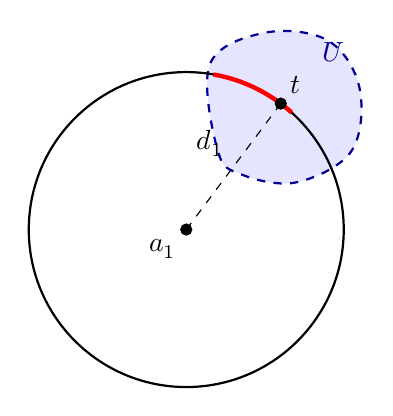
\begin{tikzpicture}
        % Define anchor point and radius
        \def\r{2}
        \coordinate (a1) at (0,0);
        \coordinate (t) at ({0.6*\r}, {0.8*\r}); % lies on the circle

        % Draw open set as a filled, irregular blob using a closed Bezier curve
        % centered roughly around t = (1.2, 1.6)
        \begin{scope}
            \clip plot[smooth cycle, tension=0.6] coordinates {
                (0.4, 1.0)
                (0.7, 0.7)
                (1.4, 0.6)
                (2.1, 1.0)
                (2.2, 1.8)
                (1.8, 2.4)
                (1.0, 2.5)
                (0.3, 2.1)
            };
            \fill[blue!10] (-3,-3) rectangle (4,4);
        \end{scope}
        \draw[blue!60!black, thick, dashed]
            plot[smooth cycle, tension=0.6] coordinates {
            (0.4, 1.0)
            (0.7, 0.7)
            (1.4, 0.6)
            (2.1, 1.0)
            (2.2, 1.8)
            (1.8, 2.4)
            (1.0, 2.5)
            (0.3, 2.1)
        };
        % Label the open set
        \node[blue!60!black] at (1.85, 2.25) {$U$};

        % Draw circle
        \draw[thick] (a1) circle (\r);

        % Highlighted open arc inside U: approximately from 48 deg to 80 deg
        \draw[red, ultra thick] ({(\r)*cos(48)}, {(\r)*sin(48)})
            arc[start angle=48, end angle=80, radius=\r];

        % Draw dashed radius line
        \draw[dashed] (a1) -- (t) node[midway, above left] {$d_1$};

        % Draw anchor point
        \filldraw (a1) circle (2pt) node[below left] {$a_1$};

        % Draw target point
        \filldraw (t) circle (2pt) node[above right] {$t$};
    \end{tikzpicture}
    \caption{The target $t$ lies in the open set $U$, and the arc $S^1(a_1,d_1)\cap U$ --- in red --- is an open arc of the circle contained in $U$, giving rise to an infinite number of candidate solutions to the positioning problem.}
    \label{fig:single-anchor}
\end{figure}


\subsubsection{The case of $n=m$}
In the event of the addition of an extra anchor point, the problem becomes conditionally solvable. To demonstrate, we begin by introducing the notion of affine independence.

\begin{Definition}
Let $p\leq q+1$. We say that $u_1, \dots, u_p\in\bR^q$ are affinely independent for if, for any coefficients $\lambda_1, \dots, \lambda_p\in\bR$:
\[
    \left(\sum_{k=1}^p \lambda_k u_k = 0, \quad \sum_{k=1}^p \lambda_k = 0\right) \implies \lambda_k = 0, \forall 1\leq k\leq p
\]
\end{Definition}

In simpler terms, a collection of $p$ vectors is said to be affinely independent if there exists no one $(p-2)$-dimensional (or lower) hyperplane on which they all lie. This is a generalization of the notion of non-collinearity ($p=3$) and non-coplanarity ($p=4$).

We now make use of the following lemma.

\begin{Lemma}
    Let $c_1, \dots, c_p\in\bR^p$ be affinely independent, and $d_1, \dots, d_p>0$. Then the spheres $S^{p-1}(c_k,d_k)$ intersect at two points at most. Moreover, said two points are reflections of each other with respect to the hyperplane spanning $c_1,\dots,c_p$.
\end{Lemma}

\begin{proof}
Let $S = \bigcap_{k=1}^p S_p(a_k, d_k)$. $S$ is characterized by the following system of equations:
\[
\begin{cases}
    \Vert x-a_1\Vert^2 = d_1^2 \qquad &(1) \\
    \qquad \vdots \\
    \Vert x-a_p\Vert^2 = d_p^2 \qquad &(p) \\
\end{cases}
\]

By considering, for every $k>1$, the equation $(1) - (k)$, we can construct a new system of equations that is linear:
\[
    d_1^2 - d_k^2 = \Vert x-a_1\Vert^2 - \Vert x-a_k\Vert^2 = \Vert a_1\Vert^2 - \Vert a_k\Vert^2 + 2\langle x, a_k-a_1\rangle \iff \langle x, a_k-a_1\rangle = C_k
\]
with $C_k := \frac{1}{2}(d_1^2 - d_k^2 + \Vert a_k\Vert^2 - \Vert a_1\Vert^2)$. In matrix form:
\[
\underbrace{
\begin{bmatrix}
    (a_2 - a_1)^T \\
    \vdots \\
    (a_p - a_1)^T
\end{bmatrix}}_A x =
\underbrace{
\begin{bmatrix}
    C_2 \\
    \vdots \\
    C_m
\end{bmatrix}}_b
\]

$A$ is a function from $\bR^p$ to $\bR^{p-1}$, and we show that its rows are linearly independent. Let $\lambda_k\in\bR$, such that:
\[
    0 = \sum_{k=2}^p \lambda_k (a_k - a_1) =  \sum_{k=2}^p \lambda_k a_k - \left(\sum_{k=2}^p \lambda_k\right)a_1
\]
Letting $\mu_1 = -\sum \lambda_k$ and $\mu_k = \lambda_k$ for $k\geq 2$, we have:
\[
    \sum_{k=1}^p \mu_k a_k = 0, \qquad \sum_{k=1}^p \mu_k = 0
\]
Invoking affine independence of $a_1,\dots,a_p$ we conclude that $\mu_k = 0$, and therefore $\lambda_k = 0$. The rows $a_k - a_1$ are hence linearly independent, and $A$ is of maximal rank $p-1$.

\begin{figure}[ht]
    \centering
    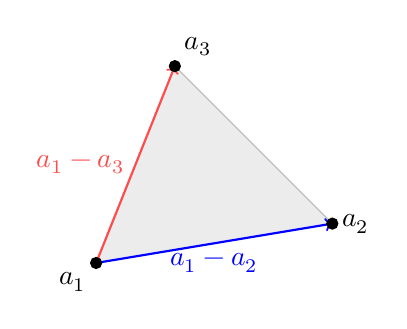
\begin{tikzpicture}
        % Anchor points
        \coordinate (a1) at (0, 0);
        \coordinate (a2) at (3, 0.5);
        \coordinate (a3) at (1, 2.5);

        % Shaded triangle (non-collinear region)
        \fill[gray!15] (a1) -- (a2) -- (a3) -- cycle;
        \draw[gray!50] (a1) -- (a2) -- (a3) -- cycle;

        % Edge vectors from a1
        \draw[->, thick, blue]   (a1) -- (a2) node[midway, below] {$a_1 - a_2$};
        \draw[->, thick, red!70] (a1) -- (a3) node[midway, left]  {$a_1 - a_3$};

        % Anchor points
        \filldraw (a1) circle (2pt) node[below left]  {$a_1$};
        \filldraw (a2) circle (2pt) node[right]       {$a_2$};
        \filldraw (a3) circle (2pt) node[above right] {$a_3$};
    \end{tikzpicture}
    \caption{Three non-collinear points in $\bR^3$ yield two linearly independent vectors $a_1 - a_2$ and $a_1 - a_3$, spanning a plane.}
    \label{fig:anchors-2d}
\end{figure}

By the rank-nullity theorem, $\dim\ker A = p - (p-1) = 1$; a straight line. Hence the equation $Ax = b$ characterizes a straight line $L$ embedded in $\bR^p$.

As a line intersects a sphere at two points at most, its intersection with $S$ will naturally not exceed that. As $x\in S \implies x\in L$, we have $S\cap L = S$, and $S$ consists of at most two points.

Now let $H$ be the hyperplane passing through all the points $a_1, \dots, a_p$. Let $\vphi:\bR^p\to\bR^p$ be the reflection map perpendicular to $H$ (figure 3).

\begin{figure}[ht]
    \centering
    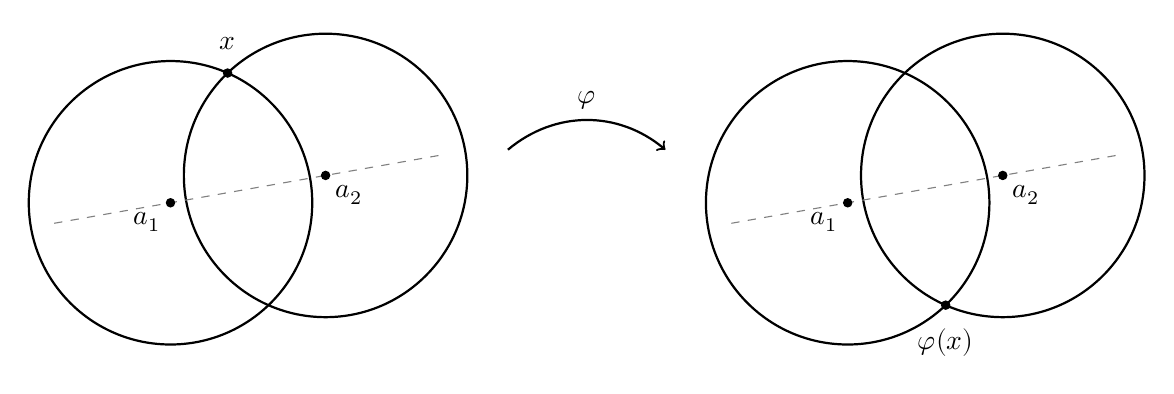
\begin{tikzpicture}[scale=1]
        % --- LEFT panel ---
        \begin{scope}[xshift=-4.3cm]
            \draw[thick] (-0.9848,-0.1736) circle (1.8);
            \draw[thick] ( 0.9848, 0.1736) circle (1.8);
            \draw[gray, dashed] (-2.462,-0.434) -- (2.462,0.434);
            \filldraw (-0.9848,-0.1736) circle (1.5pt) node[below left]  {$a_1$};
            \filldraw ( 0.9848, 0.1736) circle (1.5pt) node[below right] {$a_2$};
            \filldraw (-0.2599, 1.4739) circle (1.5pt) node[above=5pt] {$x$};
        \end{scope}

        % --- CURVED ARROW ---
        \draw[->, thick] (-1, 0.5) to[out=40, in=140] node[above] {$\varphi$} (1, 0.5);

        % --- RIGHT panel ---
        \begin{scope}[xshift=4.3cm]
            \draw[thick] (-0.9848,-0.1736) circle (1.8);
            \draw[thick] ( 0.9848, 0.1736) circle (1.8);
            \draw[gray, dashed] (-2.462,-0.434) -- (2.462,0.434);
            \filldraw (-0.9848,-0.1736) circle (1.5pt) node[below left]  {$a_1$};
            \filldraw ( 0.9848, 0.1736) circle (1.5pt) node[below right] {$a_2$};
            \filldraw ( 0.2599,-1.4739) circle (1.5pt) node[below=5pt] {$\varphi(x)$};
        \end{scope}
    \end{tikzpicture}
    \caption{The action of the reflection map $\vphi$.}
    \label{fig:reflection-map}
\end{figure}

Since $a_k\in H$, we have $\vphi(a_k)=a_k$. Moreover, as an isometry, it is norm preserving, and therefore sphere preserving:
\[
    \vphi(S_p(a_k,d_k)) = S_p(a_k,d_k) \implies \vphi(S) \subset S
\]

Thus, if the spheres intersect at $x$, they must also intersect at $\vphi(x)$. When $x\in H$, $x=\vphi(x)$, so it is only natural. When $x\notin H$, this is precisely when $S$ consists of exactly two points, reflections of each other with respect to $H$.
\end{proof}

Given that the distances we're working with are \textit{a priori} known to define a system with an existing solution, we are always looking at the case of a single, or two candidate solutions. Moreoever, making use of the reflection property, it becomes possible to determine the target $t$ uniquely, given extra assumptions about the positioning region.

In particular, letting $H_1,H_2$ be the two open half-planes split by $H$, if the positioning region is entirely contained within either of $H_1$ or $H_2$, then the problem is solvable.

For example, in a 2D RTLS deployed in a square room, two anchors can be setup at two corners of one same wall, with an associated coordinate system such that the anchors are $(0,0)$ and $(1,0)$. Then $H=\{y=0\}$, and the room lies entirely in the half-plane $H_1=\{y>0\}$. We can then uniquely solve for $t=(x,y)$ given $d_1$ and $d_2$:
\[
\begin{cases}
    x = \frac{1}{2}(d_1^2 - d_2^2 + 1) \\
    y = \sqrt{d_1^2 - x^2}
\end{cases}
\]

Likewise, in a 3D RTLS deployed in a cube room, three anchors can be setup at three corners of the floor, with an associated coordinate system such that the anchors are $(0,0,0)$, $(1,0,0)$ and $(0,1,0)$. Then $H=\{z=0\}$, and the room lies entirely in the half-plane $H_1=\{z > 0\}$. We can then solve for $t=(x,y,z)$ given $d_1, d_2, d_3$:
\[
\begin{cases}
    x = \frac{1}{2}(d_1^2 - d_2^2 + 1) \\
    y = \frac{1}{2}(d_1^2 - d_3^2 + 1) \\
    z = \sqrt{d_1^2 - x^2 - y^2}
\end{cases}
\]

\subsubsection{The case of $n=m+1$}
Once the number of anchors exceeds the dimension of the ambient space, the constraints on the geometry can be relaxed, thanks to the following lemma.

\begin{Lemma}
    Let $c_1, \dots, c_{p+1}\in\bR^p$ be affinely independent, and $d_1, \dots, d_{p+1} > 0$. Then the spheres $S^{p-1}(c_k,d_k)$ intersect at at most one point.
\end{Lemma}

\begin{proof}
Reconstructing the --- now expanded --- matrix of edges $a_1-a_k$ from the previous proof, with the corresponding constants $C_k$, we obtain a function $A$ from $\bR^p$ to $\bR^p$.
\[
\underbrace{
\begin{bmatrix}
    (a_1 - a_2)^T \\
    \vdots \\
    (a_1 - a_{p+1})^T
\end{bmatrix}}_A x =
\underbrace{
\begin{bmatrix}
    C_2 \\
    \vdots \\
    C_{p+1}
\end{bmatrix}}_b
\]

In this manner, $x$ is unique iff $A$ is invertible. As in the proof of the previous lemma, affine independence of the points $a_k$ yields linear independence of the rows $a_1-a_k$ of $A$, and hence $x$ is indeed unique.

However, though the intersection points of the spheres are necessarily solutions of $Ax=b$, the opposite is not necessarily true. Even if $x$ exists, the spheres won't necessarily intersect at all --- though if they do, it must be at $x$.

Thus the spheres intersect at at most one point.
\end{proof}

Again, by assumption, the values $d_k$ are the true distances from $t$ to the anchors $a_k$, and hence we are always looking at the case where the spheres do intersect, and $t$ is uniquely recoverable as $A^{-1}b$.

For example, in a 2D RTLS where the anchors are modeled as $(0,0), (1,0)$ and $(0,1)$, we have $A=I_2$, and hence:
\[
    t = y 
\]
Likewise in a 3D RTLS with the anchors modeled as the points $(0,0,0)$, $(1,0,0)$, $(0,1,0)$ and $(0,0,1)$; as we again have $A=I_3$.

\subsubsection{The case of $n>m+1$}
As we just established, it suffices to add one anchor above the dimension of the ambient space to be able to uniquely recover the target point. Naturally, then, adding on more anchor points will not take that away. However, it is not without benefit, in practice, to construct an over-determined system --- as we will discuss in section 3.2 ---, and so we present here one possible strategy that makes use of the excess information.

Just as previously, we construct the --- yet again expanded --- matrix of edges $A$ and vector of coefficients $b$. Recall that $Ax=b\iff Ax-b=0 \iff \Vert Ax-b\Vert=0$. This allows us to make use of linear least squares.

\begin{Theorem}
Let $A\in \bR^{p\times q}$ and $b\in\bR^p$ with $p<q$.

If $A$ is of maximal rank, then the function $f:x\mapsto \Vert Ax-b\Vert^2$ has a unique global minimizer, and:
\[
    \argmin_{x\in\bR^p} f(x) = (A^TA)^{-1}A^Tb
\]
\end{Theorem}

\begin{proof}
As a polynomial function, $f$ is $C^\infty$, and hence in particular twice-differentiable. Letting $x,h\in\bR^p$:
\[
    f(x+h) = \Vert Ax-b + Ah\Vert^2 = f(x) + 2\langle Ax-b,Ah \rangle + \Vert Ah\Vert^2
\]
Notice that $\vphi(x)(u) = 2\langle Ax-b, Au\rangle$ is linear, and $\psi(x)(u,v) = \langle Au,Av\rangle$ is bilinear, and the above equation can be rewritten as:
\[
    f(x+h) = f(x) + \vphi(x)(h) + \psi(x)(h,h)
\]

Hence $Df(x) = \vphi(x)$ and $D^2f(x) = \psi(x)$. The corresponding gradient and Hessian are:
\[
    \nabla f(x) = 2(A^TAx - A^Tb), \qquad Hf(x) = A^TA
\]

To demonstrate that $f$ has at most one minimizer, we show that $Hf(x)$ is positive definite for all $x\in\bR^p$, and hence strictly convex. Let $u\in\bR^p$:
\[
    \langle Hf(x)u, u\rangle = \langle A^TAu, u\rangle = \Vert Au\Vert^2
\]

Since $p<q$, and $A$ is of maximal rank, we have that $\dim\ker A = 0$, and hence $\Vert Au\Vert^2 > 0$ for any $u\neq 0$. Thus $Hf(x)=A^TA$ is positive definite for every $x$.

To show that a minimizer exists, we must show that $\nabla f(x) = 0$ for some $x$. First, as $A^TA$ is square and positive definite, it's invertible. Then:
\[
    \nabla f(x) = 0
    \iff A^TAx - A^Tb = 0
    \iff x = (A^TA)^{-1}A^Tb
\]

Thus $f$ has a unique global minimizer, given by $(A^TA)^{-1}A^Tb$.
\end{proof}

For our use case, the condition that $A$ be of maximal rank is fulfilled by having $(m+1)$-many of the anchors be affinely independent, and then labeling them as $a_1,\dots,a_{m+1}$, before constructing our system.

%------ STOPPED EDITING HERE ------%

\subsection{Working with Error-Prone Measurements}
Due to limited instrumental precision, as well as uncontrollable environmental factors, the measured distances we work with are almost always not the true ones. As a result, discrepancies in distance measurements will naturally result in discrepancies in the predicted position -- the extent of which depends on the approach taken.

To account for this fact in our model, the distances $d_k$ will be interpreted as random variables, the means thereof being the true distances $\widetilde d_k$ we seek to identify. For simplicity, we will assume that such random variables are Gaussian, with known variances $\sigma_k$, and independent. Equivalently, we can write:
\[
    d_k = \widetilde d_k + \sigma_k w_k, \qquad w_k\sim \mathcal N(0,1)
\]
with $w_1, \dots, w_n$ all independent.

In an indoors setting, we may further assume that said variances are equal -- and we will denote their common value $\sigma$ --, due to the anchors being identical in composition and environmental factors:
\[
    d_k = \widetilde d_k + \sigma w_k, \qquad w_k\sim \mathcal N(0,1)
\]

Let us begin by first evaluating the performances of our previously developed strategies in light of such a model. Once that's done, we will explore strategies specifically designed for solving this problem.

\subsubsection{Trilateration}
By trilateration, we refer to the strategy employed in 2.3. We will denote by $C_k$ the (random) coefficients defined within that subsection, and by $\widetilde C_k$ the alternative coefficients obtained by replacing $d_k$ with $\widetilde d_k$ in the definition:
\begin{align*}
    C_k &= \frac{1}{2} (d_1^2 - d_k^2 + \Vert a_k\Vert^2 - \Vert a_1\Vert^2) \\
    \widetilde C_k &= \frac{1}{2} (\widetilde d_1^2 - \widetilde d_k^2 + \Vert a_k\Vert^2 - \Vert a_1\Vert^2)
\end{align*}

We proceed to define the corresponding vectors:
\[
    y=
    \begin{bmatrix}
        C_2 \\ \vdots \\ C_{m+1}
    \end{bmatrix}, \qquad
    \widetilde y=
    \begin{bmatrix}
        \widetilde C_2 \\ \vdots \\ \widetilde C_{m+1}
    \end{bmatrix}
\]

Recalling that $t = T^{-1}\widetilde y$, our goal is to study the following random variable:
\[
    T^{-1}y
\]
Element-wise, we have:
\[
    C_k - \widetilde C_k = \frac{1}{2}(d_1^2 - \widetilde d_1^2) - \frac{1}{2}(d_k^2 - \widetilde d_k^2) = \frac{1}{2}\sigma_1^2 w_1^2 + \sigma_1\widetilde d_1 w_1 - \frac{1}{2}\sigma_k^2 w_k^2 - \sigma_k\widetilde d_k w_k
\]

As $w_1$ and $w_k$ are both centered, and by linearity of the expectation operator, we obtain the following:
\begin{align*}
    &\bE[C_k - \widetilde C_k] = \frac{1}{2}\left(\sigma_1^2\bE[w_1^2] - \sigma_k^2\bE[w_k^2]\right) = \frac{1}{2}(\sigma_1^2 - \sigma_k^2) \\
    &\implies \bE\left[T^{-1}y - t\right] = \bE\left[T^{-1}(y-\widetilde y) \right] = \frac{1}{2}T^{-1}
    \begin{bmatrix}
        \sigma_1^2 - \sigma_2^2 \\
        \vdots \\
        \sigma_1^2 - \sigma_{m+1}^2
    \end{bmatrix}
\end{align*}

In particular, this is an unbiased estimator iff the variances are all equal. Moreover, in that case:
\begin{align*}
    \Sigma := \mathrm{Var}\left(T^{-1}y\right)
    &= \bE\left[(T^{-1}y - t)(T^{-1}y - t)^T\right] \\
    &= \bE\left[\left(T^{-1}(y-\widetilde y)\right)\left(T^{-1}(y-\widetilde y)\right)^T\right] \\
    &= T^{-1}\bE\left[(y-\widetilde y)(y-\widetilde y)^T\right](T^{-1})^T
\end{align*}
Notice that $\bE\left[(y-\widetilde y)(y-\widetilde y)^T\right]$ is exactly the matrix of covariances of the coefficients $C_k$. Note that for $i\neq j$, $\bE[w_i^aw_j^b]=\bE[w_i^a]\bE[w_j^b]$ by independence of $w_i$ and $w_j$. We can then show that:
\begin{align*}
    \mathrm{Cov}(C_i,C_j) = \frac{\sigma^4}{2} + \sigma^2\widetilde d_1^2 \\
    \mathrm{Var}(C_i) = \sigma^4 + \sigma^2(\widetilde d_1^2 + \widetilde d_i^2)
\end{align*}

Observe that different choices of labeling the anchors will yield different variances and covariances; and in particular, picking $a_1$ to be the anchor closest to $t$ will yield the most accurate estimator comparatively. Moreover, as the variances evolve quadratically with the corresponding distances, the system is less and less robust as the target travels farther and farther away from the anchors.

Building off of this, in the trilateration-based subdivision strategy evoked in 2.4.1, we can speculate that the subdivision yielding the most accurate positioning will almost surely be the one closest -- in the mean squared sense -- to the target, with the convention that $a_1$ is the anchor that's closest among them.

\subsubsection{Linear Ordinary Least Squares}
We carry over the notation $C_k$ and $\widetilde C_k$ from the previous subsection, and $A$ from 2.4.2. We let:
\[
    b=
    \begin{bmatrix}
        C_2 \\ \vdots \\ C_n
    \end{bmatrix}, \qquad
    \widetilde b=
    \begin{bmatrix}
        \widetilde C_2 \\ \vdots \\ \widetilde C_n
    \end{bmatrix}
\]

Recalling that $t=(A^TA)^{-1}A^T\widetilde b$, our goal is to study the following random variable:
\[
    \hat t_\text{OLS} := (A^TA)^{-1}A^Tb
\]
to determine how good of an estimator it is for $t$.

Firstly, $\hat t_\text{OLS}$ can be unbiased even if the variances are not all equal. To demonstrate this, observe that we have:
\[
    \bE[\hat t_\text{OLS}-t] = (A^TA)^{-1}A^T\bE[b-\widetilde b]
\]

For this quantity to be null, it must be that $A^T\bE[b-\widetilde b] = 0$. Yet, $A$ is of maximal rank $m$, and the ranks of a matrix and its transpose are always equal, and hence:
\[
    \dim\ker A^T = (n-1) - \dim\mathrm{Im}\, A^T = n-1-m > 0
\]

We obtain the covariance matrix like so:
\begin{align*}
    \Sigma_\text{LS} := \mathrm{Var}(\hat t_\text{OLS})
    &= \bE\left[(\hat t_\text{OLS} - t)(\hat t_\text{OLS} - t)^T \right] \\
    &= \bE\left[\left((A^TA)^{-1}A^T(b-\widetilde b)\right)\left((A^TA)^{-1}A^T(b-\widetilde b)\right)^T \right] \\
    &= N\bE\left[(b-\widetilde b)(b-\widetilde b)^T\right]N^T
\end{align*}
where we denote $N := (A^TA)^{-1}A^T$. In particular, when $\bE[b]=\widetilde b$, then just as in trilateration, $\bE\left[(b-\widetilde b)(b-\widetilde b)^T\right]$ is exactly $\mathrm{Var}(b)$; the matrix of covariances of the coefficients $C_k$. Note that this matrix is positive definite, as we established earlier that its entries are all strictly positive. Moreover, it's symmetric.

Notice then that the average variance of said coefficients is not necessarily lower than the average obtained from only considering the coefficients upto $C_{m+1}$; for example, if $\widetilde d_{m+2} > \widetilde d_k$ for all $2 \leq k\leq m+1$, this will naturally cause the average of $C_2, \dots, C_{m+1}, C_{m+2}$ to increase. So the least squares estimator is not necessarily more advantageous in terms of its covariance properties.

However, it remains a more robust strategy compared to trilateration due to its ability to retain an unbiased estimator in the face of non-homoscedas-tic noise (i.e. when the variances $\sigma_k^2$ are not all equal) in some configurations (i.e. as long as $\bE[b]$ lies in some hyperplane containing $\widetilde b$).

This leads us straight into the first of the dedicated strategies.

\subsubsection{Linear Generalized Least Squares}
In the generalized least squares strategy, we modify our objective function in order to take into account the probabilistic model's properties.

Let $A,b,\widetilde b$ be as in the previous subsection, and let $\Psi = \mathrm{Var}(b)$. We seek to find the minimizer of the following function:
\[
    g(x) = (Ax-b)^T\Psi^{-1}(Ax-b)
\]

We show that $g$ is strictly convex. Let $x,h\in\bR^m$:
\[
    g(x+h) = g(x) + 2\langle A^T\Psi^{-1}(Ax-b), h\rangle + \langle h, A^T\Psi^{-1}Ah\rangle
\]

Let $\vphi(x)(u) = 2\langle A^T\Psi^{-1}(Ax-b), u\rangle$, and $\psi(x)(u,v) = \langle u, A^T\Psi^{-1}Av\rangle$. Then $\vphi(x)$ is linear, and $\psi(x)$ is bilinear; for every $x$. Hence $g$ is twice-differentia-ble, and we have:
\[
    g(x+h) = g(x) + \vphi(x)(h) + \psi(x)(h,h)
\]
Equivalently:
\[
    \nabla g(x) = 2A^T\Psi^{-1}(Ax-b), \qquad
    Hg(x) = A^T\Psi^{-1}A
\]

To see that $Hg(x)$ is positive definite, simply observe that the map $\eta:u\mapsto u^T\Psi^{-1}u$ defines a norm on $\bR^m$, and $\langle Hg(x)u,u\rangle = \eta(Au)$. Recalling the assumption that $A$ is of maximal rank, we conclude that $\eta(Au)>0$ for $u\neq 0$. Hence $g$ is strictly convex. We now attempt to find its minimizer:
\begin{align*}
    \nabla g(x) = 2A^T\Psi^{-1}(Ax-b) = 0 \\
    \iff x = (A^T\Psi^{-1}A)^{-1}A^T\Psi^{-1}b
\end{align*}
We label this quantity $\hat t_\text{GLS}$.

Notice that had we replaced $b$ with $\widetilde b$, we would have $At-\widetilde b=0$ and hence naturally $2A^T\Psi^{-1}(At-\widetilde b) = 0$. As a consequence:
\[
    t = (A^T\Psi^{-1}A)^{-1}A^T\Psi^{-1}\widetilde b
\]

As usual, we begin by checking whether $\hat t_\text{GLS}$ is unbiased:
\[
    \bE[\hat t_\text{GLS} - t] = (A^T\Psi^{-1}A)^{-1}A^T\Psi^{-1}\bE[b-\widetilde b]
\]
As $\Psi^{-1}$ is an automorphism, it does not add any more degrees of freedom for the choice of $\bE[b]$, but simply transforms the previous $(n-1-m)$-dimensional hyperplane into a new one of the same dimension, also containing $\widetilde b$. In this aspect, the generalized least squares estimator is no better or worse than the ordinary least squares one.

Let us now examine its covariace matrix in the absence of bias:
{\hfuzz=\maxdimen
\begin{align*}
    \Sigma_\text{GLS} := \mathrm{Var}(\hat t_\text{GLS})
    &= (A^T\Psi^{-1}A)^{-1}A^T\Psi^{-1}\bE[(b-\widetilde b)(b-\widetilde b)^T]\Psi^{-1}A(A^T\Psi^{-1}A)^{-1} \\
    &= (A^T\Psi^{-1}A)^{-1}(A^T\Psi^{-1}A)(A^T\Psi^{-1}A)^{-1} \\
    &= (A^T\Psi^{-1}A)^{-1}
\end{align*}
}

To demonstrate that $\hat t_\text{GLS}$ is indeed more optimal than $\hat t_\text{OLS}$, we begin by introducing our metric for comparison.

\begin{Definition}
Let $O(p)$ be the set of symmetric $p\times p$ matrices. We define a partial ordering $\preceq$ on $O(p)$ like so:
\[
    A,B\in O(p), \quad A\preceq B \iff B-A \text{ is positive semi-definite}
\]
We call this ordering in the positive semi-definite (PSD) sense. 
\end{Definition}

Note that $A\preceq B$ in this sense is equivalent to all eigenvalues of $A$ being less than or equal to the eigenvalues of $B$, hence why it makes sense to use this as a metric for comparison. We now define the OLS-GLS difference matrix:
\[
    M = (A^TA)^{-1}A^T - (A^T\Psi^{-1}A)^{-1}A^T\Psi^{-1}
\]
Then $\hat t_\text{OLS} = \hat t_\text{GLS} + Mb$. Moreover, $\hat t_\text{GLS}$ and $Mb$ are uncorrelated:
\begin{align*}
    \mathrm{Cov}(\hat t_\text{GLS}, Mb)
    &= \bE\left[(Lb-L\widetilde b)(Mb-M\widetilde b)^T\right] \\
    &= \bE\left[L(b-\widetilde b)(b-\widetilde b)^TM^T\right] \\
    &= L\Psi M^T
\end{align*}
where $L := (A^T\Psi^{-1}A)^{-1}A^T\Psi^{-1}$. Let's compute this quantity:
\begin{align*}
    L\Psi M^T
    &= (A^T\Psi^{-1}A)^{-1}A^T\Psi^{-1}\Psi\left[A(A^TA)^{-1} - \Psi^{-1}A(A^T\Psi^{-1}A)^{-1} \right] \\
    &= (A^T\Psi^{-1}A)^{-1} - (A^T\Psi^{-1}A)^{-1} \\
    &= 0
\end{align*}

And hence:
\[
    \Sigma_\text{OLS} = \Sigma_\text{GLS} + \mathrm{Var}(Mb) = \Sigma_\text{GLS} + M\Psi M^T \iff \Sigma_\text{OLS} - \Sigma_\text{GLS} = M\Psi M^T
\]

As $\zeta: u\mapsto u^T\Psi u$ defines a norm on $\bR^m$, $\langle M\Psi M^Tu, u\rangle = \zeta(M^Tu) \geq 0$ and hence $M\Psi M^T$ is positive semi-definite. Thus $\Sigma_\text{GLS} \preceq \Sigma_\text{OLS}$.

In fact, this result can be further generalized via the Gauss-Markov theorem to yield that $\hat t_\text{GLS}$ is the best unbiased linear estimator of $t$ in terms of $b$, when $\bE[b]=\widetilde b$.

\begin{Theorem}
Let $X\in\bR^{p\times q},\beta\in\bR^q$, let $\alpha$ be an $\bR^p$-valued random variable, and let $\eps$ be an $\bR^q$-valued random variable, with $\bE[\eps]=0$ and $\mathrm{Var}(\eps)=\sigma^2 I$ for some $\sigma>0$; such that
\[
    \alpha = X\beta + \eps
\]

Let $\hat \beta = (X^TX)^{-1}X^T\alpha$ and $\bar \beta = T\alpha$ be two unbiased estimators of $\beta$; with $T\in\bR^{p\times q}$. Then:
\[
    \mathrm{Var}(\hat\beta) \preceq \mathrm{Var}(\bar\beta)
\]
\end{Theorem}

Though this seems to suggest that $\hat t_\text{OLS}$ is the best estimator, recall that in our model $b = \widetilde b + (b-\widetilde b) = At + (b-\widetilde b)$, and yet $\mathrm{Var}(b-\widetilde b)=\mathrm{Var}(b)$ is not a scalar multiple of the identity. The theorem is not directly applicable yet.

In order to make it so, it suffices to multiply both sides of the equation by $\Psi^{-1/2}$:
\[
    \Psi^{-1/2}b = \Psi^{-1/2}At + \Psi^{-1/2}(b-\widetilde b)
\]
the matrix $\Psi^{-1/2}$ being well-defined as $\Psi$ is positive definite; moreover, it's positive definite and symmetric. In this manner:
\[
    \mathrm{Var}(\Psi^{-1/2}b) = \Psi^{-1/2}\mathrm{Var}(b)\Psi^{-1/2} = \Psi^{-1/2}\Psi\Psi^{-1/2} = I
\]

Applying the Gauss-Markov theorem with $X:=\Psi^{-1/2}A$ and $\alpha:=\Psi^{-1/2}b$ now, we obtain the best unbiased linear estimator for $t$:
\[
    (A^T\Psi^{-1/2}\Psi^{-1/2}A)^{-1}A^T\Psi^{-1/2}\Psi^{-1/2}b = \hat t_\text{GLS}
\]

Now, this yields that $\hat t_\text{GLS}$ is the best unbiased linear estimator in terms of $\Psi^{-1/2}b$, but in fact any linear estimator of the form $Xb$ can be rewritten as $X\Psi^{1/2}(\Psi^{-1/2}b)$, where $X$ is a matrix; and hence $\hat t_\text{GLS}$ is in fact the best unbiased linear estimator of $t$ in terms of $b$.

Moreover, if we let $P$ be the standard projection from $\bR^{n-1}$ to $\bR^{m}$, then we have $y=Pb$. Hence, $\hat t_\text{tri}=T^{-1}Pb$ is unbiased and linear in $b$ and thus $\Sigma_\text{tri}\succeq \Sigma_\text{GLS}$.

\subsubsection{Estimating $\Psi$}
The biggest hurdle with using the generalized least squares strategy is that it presupposes knowledge of the covariance matrix $\Psi$. However, as previously established, the entries of this matrix depend on the true distances $\widetilde d_k$, which are unknown to us in practice.

\vskip .3cm
\noindent
\textbf{Feasible Generalized Least Squares}

\noindent
A first strategy for handling this problem is the Feasible Generalized Least Squares (FGLS): as we had previously assumed the measured distances $d_k$ to have mean $\widetilde d_k$, the former are naturally unbiased estimators of the latter. Hence, by replacing $\widetilde d_k$ in $\Psi$ with $d_k$, we obtain an estimator $\hat\Psi$ of $\Psi$:
\[
    \hat\Psi_{ij}=\frac{\sigma^4}{2}+\sigma^2 d_1^2, \qquad
    \hat\Psi_{ii}=\sigma^4+\sigma^2(d_1^2 + d_i^2), \qquad \forall i\neq j
\]

Though this is the easiest strategy in terms of computational cost, it is heavily flawed, as the estimator is biased:
\[
    \bE[d_k^2] = \widetilde d_k^2 + \sigma^2\bE[w_k^2] = \widetilde d_k^2 + \sigma^2
\]

\vskip .3cm
\noindent
\textbf{Iteratively Reweighted Least Squares}

\noindent
A second strategy is the Iteratively Reweighted Least Squares (IRLS). As the name indicates, this strategy aims to iteratively improve upon the estimator:
\begin{enumerate}
    \item On the first iteration: Perform OLS to obtain the first estimator $\hat t^{(1)}$ for $t$. Compute the distances $d_k^{(1)} = \Vert \hat t^{(1)} - a_k\Vert$. Construct $\hat\Psi^{(1)}$ from the obtained distances.
    \item On the $(i+1)$-th iteration: Use $\hat\Psi^{(i)}$ to perform GLS and obtain the estimator $\hat t^{(i+1)}$ for $t$. Compute the distances $d_k^{(i+1)} = \Vert \hat t^{(i+1)} - a_k\Vert$. Construct $\hat\Psi^{(i+1)}$ from the obtained distances.
    \item Stop when the desired degree of convergence is achieved.
\end{enumerate}

An exact evaluation of the performance of the thus produced estimator $\hat t^{(n)}$ is difficult to produce. Though the third step implicitly assumes it, and intuitively, it makes sense to think that $\hat\Psi^{(n)}\to\Psi$ almost surely -- and hence $\hat t^{(n)}\to\hat t_\text{GLS}$ almost surely --, whether such is always true remains an open problem.

\subsubsection{Maximum Likelihood}
Up until now, we have only considered strategies yielding explicitly defined estimators. Though this allows for ease of computation, it limits the quality of the estimators we can work with. In particular, it is known that the best estimator there is, is that of maximum likelihood.

For clarity, we modify our previous notation to make is so $D_k$ denotes the distance random variable, and $d_k$ its observation.

Recalling that $\widetilde d_k = \Vert t-a_k\Vert$, we can write:
\[
    D_k = \Vert t-a_k\Vert + \sigma_k w_k
\]
expliciting $t$ as a parameter of the distributions of the distances $D_k$.

We seek to find the point $\hat t_\text{MLE}$ which maximizes the value of the joint probability density function of $D_1, \dots, D_n$ at their observed values $d_1, \dots, d_n$:
\[
    f(d_1, \dots, d_n; x) = \prod_{k=1}^n f(D_k=d_k;x) = \prod_{k=1}^n \frac{1}{\sqrt{2\pi}\sigma_k}\exp{\left(-\frac{(d_k-\Vert x-a_k\Vert)^2}{2\sigma_k^2}\right)}
\]

As the logarithm is increasing, maximizing $f$ is equivalent to maximizing $\log f$:
\[
    \log f(d_1, \dots, d_n;x) = -\sum_{k=1}^{n} \left(\log{\sqrt{2\pi}\sigma_k} + \frac{(d_k-\Vert x-a_k\Vert)^2}{2\sigma_k^2}\right)
\]

Notice that if we let $d = (d_1, \dots, d_n)$, $\widetilde d(x)=(\Vert x-a_1\Vert, \dots, \Vert x-a_n\Vert)$ and $S=\mathrm{diag}(\sigma_1,\dots,\sigma_n)$, then:
\[
    \sum_{k=1}^n \frac{(d_k-\Vert x-a_k\Vert)^2}{\sigma_k^2} = \Vert S(d-\widetilde d(x))\Vert^2
\]

As minimizing this quantity is equivalent to maximizing $\log f(d;x)$, we conclude on our maximum likelihood estimator:
\[
    \hat t_\text{MLE} = \argmin_{x\in\bR^m} \Vert S(d-\widetilde d(x)) \Vert^2
\]

In the homoscedastic case, when $\sigma_k=\sigma$, this reduces down further to the naive least squares:
\[
    \hat t_\text{MLE} = \argmin_{x\in\bR^m} \Vert d-\widetilde d(x)\Vert^2
\]

Given that this optimization problem is not solvable analytically, it's only ever possible to work with approximations obtained through numerical methods (e.g. gradient descent, Gauss-Newton).

\pagebreak
\noindent
Let $S = \mathrm{diag}(\sigma_1, \dots, \sigma_n), d=(d_1, \dots, d_n)$, and define the function:
\[
    \widetilde d(x) = \begin{bmatrix}
        \Vert x-a_1\Vert \\
        \vdots \\
        \Vert x-a_n\Vert
    \end{bmatrix}
\]

The MLE is obtained by solving a weighted least squares problem:
\[
    \hat t_\text{MLE} = \argmin_{x\in\bR^2} \Vert S(d-\widetilde d(x))\Vert^2 
\]

In particular, when the noise is i.i.d. (i.e., $\sigma_1=\dots=\sigma_n$), this coincides with solving the unweighted least squares problem:
\[
    \hat t_\text{MLE} = \argmin_{x\in\bR^2} \Vert d-\widetilde d(x)\Vert^2
\]

\vskip 1cm

\[
    \hat t_\text{GLS} = (A^T\Psi^{-1}A)^{-1}A^T\Psi^{-1}b, \qquad \Psi = \bE\left[(b-\widetilde b)(b-\widetilde b)^T\right]
\]


% Implementation section goes in implementation.tex
\section{Implementation}
Talk about our implementation hardware, software, architecture, etc. here...


% Results section goes in results.tex
\section{Results}

\begin{table}[ht]
\centering
\caption{MLE-4 execution time and error statistics for differing iteration counts. The execution time statistics are taken over 300 iterations, following a discarded first iteration. The error statistics are taken over 500 iterations, with simulated AWGN ($\sigma=5$) added to the input distances in mm.}
\label{tab:mle_stats}
\begin{tabular}{ccccccc}
\toprule
\multirow{2}{*}{N{\textdegree} Iterations}
  & \multicolumn{2}{c}{Execution Time (CPU cycles)}
  & \multicolumn{4}{c}{Error (mm)} \\
\cmidrule(lr){2-3} \cmidrule(lr){4-7}
  & Min & Max & Min & Max & Mean & Std.\ Dev. \\
\midrule
3 & 3009 (5.0\,\textmu s)  & 3101 (5.2\,\textmu s)  & 0.05 & 132.73 & 8.22 & 15.96 \\
4 & 3974 (6.6\,\textmu s)  & 4061 (6.8\,\textmu s)  & 0.23 &  11.91 & 4.17 &  2.28 \\
6 & 5876 (9.8\,\textmu s)  & 5992 (10.0\,\textmu s) & 0.27 &  11.91 & 4.14 &  2.23 \\
8 & 7764 (12.9\,\textmu s) & 7933 (13.2\,\textmu s) & 0.28 &  11.90 & 4.14 &  2.23 \\
\bottomrule
\end{tabular}
\end{table}

\begin{table}[ht]
\caption{MLE-3 execution time and error statistics for differing iteration counts. The execution time statistics are taken over 300 iterations, following a discarded first iteration. The error statistics are taken over 500 iterations, with simulated AWGN ($\sigma=5$) added to the input distances in mm.}
\label{tab:mle_3anchors}
\centering
\begin{tabular}{ccccccc}
\toprule
\multirow{2}{*}{N{\textdegree} Iterations}
  & \multicolumn{2}{c}{Execution Time (CPU cycles)}
  & \multicolumn{4}{c}{Error (mm)} \\
\cmidrule(lr){2-3} \cmidrule(lr){4-7}
  & Min & Max & Min & Max & Mean & Std.\ Dev. \\
\midrule
 4 &  3408 (5.7\,\textmu s) &  3493 (5.8\,\textmu s) & 0.06 & 800.55 & 13.26 & 69.77 \\
 8 &  6616 (11.0\,\textmu s) &  6795 (11.3\,\textmu s) & 0.07 &  19.45 &  2.86 &  2.57 \\
12 &  9838 (16.4\,\textmu s) & 10081 (16.8\,\textmu s) & 0.06 &  19.24 &  2.86 &  2.58 \\
16 & 13060 (21.8\,\textmu s) & 13382 (22.3\,\textmu s) & 0.06 &  19.30 &  2.86 &  2.58 \\
\bottomrule
\end{tabular}
\end{table}




\begin{table}[ht]
\caption{Execution time and error statistics for trilateration, OLS, and FGLS algorithms. The execution time statistics are taken over 300 iterations, following a discarded first iteration. The error statistics are taken over 500 iterations, with simulated AWGN ($\sigma=5$) added to the input distances in mm.}
\label{tab:exec_time}
\centering
\begin{tabular}{ccccccc}
\toprule
\multirow{2}{*}{Method}
  & \multicolumn{2}{c}{Execution Time (CPU cycles)}
  & \multicolumn{4}{c}{Error (mm)} \\
\cmidrule(lr){2-3} \cmidrule(lr){4-7}
  & Min & Max & Min & Max & Mean & Std.\ Dev. \\
\midrule
Trilateration
  & 34 (56.7\,ns) & 35 (58.3\,ns)
  & 0.02 & 23.23 & 3.47 & 0.02 \\
OLS
  & 270 (450\,ns) & 270 (450\,ns)
  & 0.04 & 15.71 & 2.68 & 2.32 \\
FGLS
  & 1074 (1.79\,\textmu s) & 1102 (1.84\,\textmu s)
  & 0.06 & 10.27 & 2.40 & 1.88 \\
\bottomrule
\end{tabular}
\end{table}


\end{document}
